\section{Introduction}

Ransomware is one of the biggest cybercrime threats of our days, both for organizations and individuals. This was again demonstrated by the recent global attack of the WannaCry trojan \cite{Symantec2017} shown in figure \ref{fig:wanna_cry}, where more than 230000 computers in 150 different countries got infected. The attack also showed that there is often still no other way for infected victims than paying the ransom, if they want to get their data back and have no sufficient Backups. Precautions like regular security updates can help to avoid the damage, but there is no waterproof solution and people working with crucial data need to be educated about the topic. Among others, the \gls{nhs} faced huge troubles through WannaCry \cite{Martin2017}, which exemplifies that wallets can be affected by ransomware as well as health conditions.

\begin{figure}[htbp]
  \begin{center}
    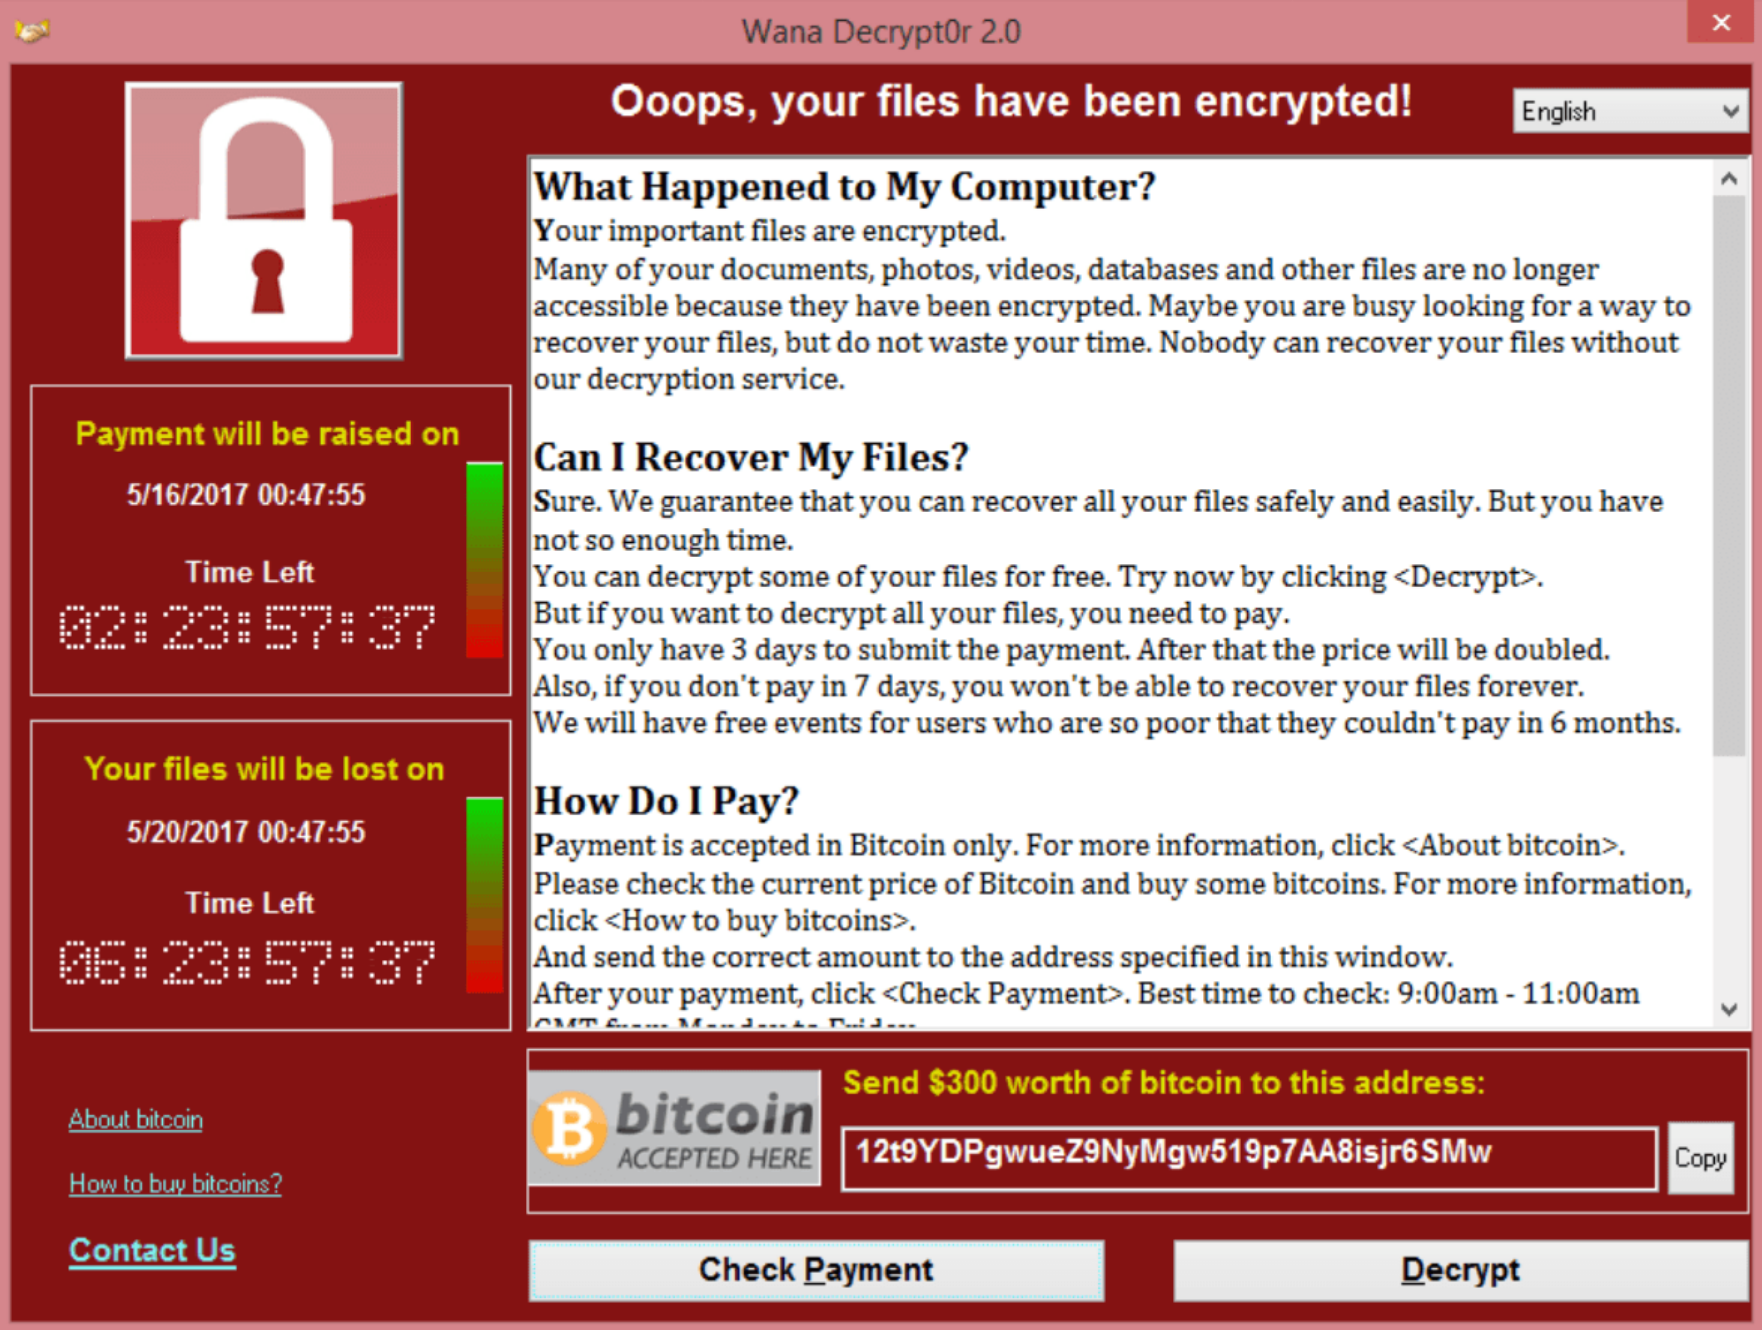
\includegraphics[width=0.8\textwidth]{images/wanna_cry.png}
    \caption{WannaCry Ransomware}
    \label{fig:wanna_cry}
  \end{center}
\end{figure}

This seminar work focuses on giving an overview of ransomware.
%TODO
